\documentclass[landscape, a4paper]{article}
\usepackage[top=0.5cm,bottom=0.5cm,left=0.5cm,right=0.5cm]{geometry}
\usepackage[export]{adjustbox}
\usepackage{ipsum}
\usepackage{xcolor}
\usepackage{caption}
\usepackage{csquotes}
\usepackage[parfill]{parskip}

\captionsetup{labelformat=empty, justification=centering, font={color=PrimaryColor}}

\definecolor{PrimaryColor}{HTML}{8FA85F}
\newcommand\alert[1]{\textcolor{PrimaryColor}{\textbf{#1}}}

\begin{document}
\footnotesize
\begin{minipage}[t]{0.32\textwidth}
	\setlength{\parskip}{0.25cm}

	\vspace{0.5cm}

		\textcolor{PrimaryColor}{
			\rule{\linewidth}{0.5mm}
			\vspace{-0.1cm}
			\begin{center}
				\large
				\textsc{Wanderung zur Burg Kybfelsen}
			\end{center}
			\rule{\linewidth}{0.5mm}
		}
		\vspace{0.15cm}

		Eine unvergessliche Wanderung durch die zauberhafte Naturlandschafft des Freiburger \alert{Günterstals} hinauf zur mysteriösen Burgruine Kybfelsen! Der Weg führt tief in die Wälder, vorbei an plätschernden Bächen, imposanten Felsen und verwunschenen Lichtungen. Schon nach den ersten Schritten taucht man in die friedvolle Stille des Schwarzwalds ein, wo man unter den mächtigen Bäumen voll und vom Wald verschluckt wird und der Hektik der Großstadt entfliehen kann.

		Das \alert{Arboretum in Günterstal} lädt zu einer Reise durch die Welt der Bäume. Dafür wurde eine Auswahl der gepflanzten Bäume und Sträucher nach Themen geordnet und mit Hinweistafeln versehen. Jeder der fünf Themenpfade ist einem Herkunftsgebiet, einer Gruppe verwandter Baumarten oder einem besonderen Aspekt der Beziehungen zwischen der Lebenswelt der Bäume und der Lebenswelt der Tiere oder Menschen gewidmet.

		\includegraphics[width=\linewidth]{./figures/arboretum.png}
		\captionof{figure}{Arboretum in Günterstal mit seinen Themenpfaden}
		\setlength{\parskip}{0.25cm}
		\vspace{0.15cm}
		Ein \alert{Arboretum} (lat.\ Nebenform zu arbustum hier speziell im Sinne von Baumpflanzung von arbor Baum) ist eine Sammlung (nicht in Pflanzgefäßen wachsender) verschiedenartiger, oft auch exotischer Gehölze; dies kann beispielsweise ein botanischer Garten sein, in dem hauptsächlich Bäume und Sträucher angepflanzt werden. Man spricht von einem Fruticetum, wenn nur Sträucher angepflanzt werden. Werden in einem Arboretum nur Nadelgehölze angepflanzt, nennt man es Pinetum.
\end{minipage}
\hspace{0.4cm}
\begin{minipage}[t]{0.32\textwidth}
	\setlength{\parskip}{0.25cm}
	Das \alert{Stadtwald-Arboretum} entstand bereits Ende des 19. Jahrhunderts, als die Freiburger Förster in stadtnahen Wäldern begannen, fremdländische Baumarten zu Versuchszwecken zu pflanzen. Jedoch gelang nur bei wenigen Baumarten die Integration in die heimische Waldgesellschaft. Das wohl berühmteste und für den Stadtwald Freiburg charakteristische Beispiel ist die forstwirtschaftliche Nutzung der nordamerikanischen Baumart Douglasie, die bereits seit 1896 in Freiburg forstwirtschaftlich genutzt wird und heute eine der wirtschaftlich wichtigsten Baumarten ist.

	\includegraphics[width=\linewidth]{./figures/waldraud.png}
	\captionof{figure}{Waldtraut vom Mühlwald --- höchster amtlich vermessener Baum Deutschlands}
	\setlength{\parskip}{0.25cm}
	\vspace{0.15cm}

	Die \alert{Douglasie} ist im Schwarzwald wirtschaftlich bedeutsam, weil sie schnell wächst, robust gegenüber Trockenheit und Schädlingen ist und qualitativ hochwertiges Holz liefert, das vielseitig genutzt werden kann. Zudem verbessert sie als Teil von Mischwäldern die Stabilität und Widerstandsfähigkeit des Waldes, was sie angesichts des Klimawandels besonders attraktiv macht.\\
	Der Name Douglasie hat übrigens nichts mit dem Parfüm- und Kosmetikunternehmen Douglas zu tun. Der Name der Douglasie leitet sich vom schottischen Botaniker David Douglas ab, der die Baumart im 19. Jahrhundert aus Nordamerika nach Europa brachte. Der Name des Unternehmens Douglas hingegen geht auf den Gründer John Sharp Douglas zurück, der 1821 eine Seifenfabrik in Hamburg eröffnete, die später zu einem Parfüm- und Kosmetikunternehmen wurde.

	Ein besonderes Highlight auf der Strecke ist \alert{Waldtraud}, die (im Jahr 2024) 114 Jahre alte Douglasie trägt mit ihren stolzen 67 Metern Höhe den Titel als höchster Baum Deutschlands. Sie wurde 1913 als dreijährige Pflanze an den jetzigen Standort etwas südlich des heutigen Arboretums Freiburg-Günterstal gesetzt.

	Die Wanderroute hält allerdings noch mehr bereit: An mehreren Aussichtspunkten kannt man atemberaubende Blicke über Freiburg und das Günterstal genießen. Neben der Landschaft erlebst man auch ein Stück Geschichte – viele berühmte Persönlichkeiten haben hier ihre Spuren hinterlassen.
\end{minipage}
\hspace{0.4cm}
\begin{minipage}[t]{0.32\textwidth}
	\setlength{\parskip}{0.25cm}

	Namentlich erwähnt wird \alert{Günterstal} zum ersten Mal in einer Besitzurkunde aus dem Jahr 804, damals als \enquote{Gundherrerhusir} (Häuser des Günther) in der Mark von Merzhausen. Rund 300 Jahre später taucht der Ort unter dem Namen \enquote{Guntheristal} wieder auf. Um 1221 schenkt ein Adeliger, der einer Überlieferung aus dem 18. Jahrhundert zufolge Günther von Kibenfels hieß seiner Tochter Adelheid das Gelände in Günterstal. Dort baut sie mit ihren Gefährtinnen eine kleine klösterliche Anlage. In einer Urkunde von 1224 wird das Kloster in \enquote{Günterstal} erstmals erwähnt. Günther von Kibenfels kann jedoch nicht der Namensgeber des Ortes sein, da der Name \enquote{Günter} schon sehr viel früher im Ortsnamen auftauchte. Auf der Wanderroute kommt man auch am Torhaus des ehemaligen Klosters vorbei, welches von Straßenbahn durchfahen wird.

	Unter anderem ist der bedeutende deutsche Mathematiker \alert{Ernst Zermelo} auf dem Friedhof in Günterstal in Freiburg beerdigt. Sein Grab liegt neben dem von Edmund Husserl. Ernst Zermelo war ein bedeutender Mathematiker, der die Mengenlehre revolutionierte. Er formulierte das Zermelo-Axiomensystem, das die Grundlage für die moderne Mengenlehre bildet. Besonders bekannt sind die \alert{Zermelo-Fraenkel-Axiome}, welche die mathematische Struktur von Mengen präzise definieren und heute in der Mathematik weit verbreitet sind. Ein weiteres wichtiges Resultat seiner Arbeit ist das Auswahlaxiom, das in vielen Bereichen der Mathematik, wie der Analysis und Algebra unerlässlich ist. Zermelos Beiträge legten die Grundlage für viele moderne mathematische Theorien.

	\includegraphics[width=\linewidth]{./figures/tor.png}
	\captionof{figure}{Torhaus des ehemaligen Klosters}
	\setlength{\parskip}{0.25cm}
	\vspace{0.15cm}

	Er arbeitete ab 1926 mit einer Ehren-Professur an der \alert{Albert-Ludwigs-Universität} in Freiburg im Breisgau, musste diese Arbeit aber 1935 wieder aufgeben, da er sich weigerte die Vorlesungen mit Hitlergruß zu beginnen, was von Kollegen (Gustav Doetsch und dessen Assistent Eugen Schlotter) denunziert wurde. Nach dem Zweiten Weltkrieg bezog er seine Position als Honorarprofessor wieder, konnte aber aufgrund seines gesundheitlichen Zustandes keine Vorlesungen mehr halten.
\end{minipage}
\newpage
\begin{minipage}[t]{0.32\textwidth}
	\vspace{0cm}
	\setlength{\parskip}{0.25cm}

	\includegraphics[width=\linewidth]{./figures/grabstein.png}
	\captionof{figure}{Grabstein von Ernst Zermelo im Friedhof Günterstal}
	\setlength{\parskip}{0.25cm}
	\vspace{0.15cm}
	Im April 2018 wurde in Freiburg ihm zu Ehren die Eckerstraße, in der sich das Mathematische Institut der Albert-Ludwigs-Universität Freiburg befindet, in \alert{Ernst-Zermelo-Straße} umbenannt. Wie das Erläuterungsschild unter dem neuen Namen erklärt, wurde die Straße aufgrund der problematischen Vorreiterrolle Alexander Eckers als völkischer Rassenideologe umbenannt. Der neue Name ist für das Institut gut ausgewählt: Ernst Zermelo ist Namensgeber der Heimatadresse des Ernst-Mach-Instituts und der Mathematikdidaktik der Universität Freiburg, beides sind Institutionen, die ohne die Zermelo’sche Mengenlehre der Mathematik wohl nicht weit kämen. % Sogar ein Himmelskörper, der Asteroid 14990 Zermelo, ist nach dem Mathematiker benannt.

	\includegraphics[width=\linewidth]{./figures/straßenschild.png}
	\captionof{figure}{Ehemalige Eckerstraße in Ernst-Zermelo-Straße umbenannt}
	\setlength{\parskip}{0.25cm}
	\vspace{0.15cm}
\end{minipage}
\hspace{0.4cm}
\begin{minipage}[t]{0.32\textwidth}
	\setlength{\parskip}{0.25cm}
	\vspace{0cm}

	Auf der Wanderroute geht es zur \alert{Burg Kybfelsen}, die geheimnisvoll zwischen den Bäumen verborgen liegt. Eine Burg auf dem Kybfelsen wird in der Chronik des Matthias von Neuenburg aus der Mitte des 14. Jahrhunderts erwähnt. Der Name \enquote{Kyburg} taucht erstmals 1484 im Weistum von Kappel auf. Erbrachtes Fundmaterial aus Grabungen an der Burgstelle in den 1920er Jahren durch Otto Kantorowicz belegen die Existenz der Anlage bereits während der Zeit der Zähringer Herrschaft im Breisgau des späten 11. bzw. frühen 12. Jahrhunderts. %Lesekeramikfunde, die sich in das 12. und frühe 13. Jahrhundert datieren lassen, vervollständigen die Sicht auf den Nutzungszeitraum des befestigten Platzes

	Der \alert{Stadtteil Zähringen} in Freiburg hat seinen Namen von der Zähringer Dynastie, einem Adelsgeschlecht, das im Mittelalter eine bedeutende Rolle in der Region spielte. Der Name \enquote{Zähringen} leitet sich von der ehemaligen Zähringer Burg ab, die im 11. Jahrhundert von den Zähringern erbaut wurde. Diese Burg lag in der Nähe des heutigen Zähringer Stadtteils und war ein strategisch wichtiger Punkt, um das Umland zu kontrollieren. Die Zähringerstraße und das Zähringer Schloss sind noch heute Zeugen dieser Geschichte.

	Die \alert{Zähringer Burg} auf dem Schlossberg verlor im 13. Jahrhundert an Bedeutung und wurde später zerstört. Heute sind nur noch wenige Reste der Burg erhalten. Die Überreste befinden sich auf dem Zähringer Berg im Stadtteil Zähringen, wo man noch die Grundmauern und Teile der ehemaligen Burganlage finden kann.

	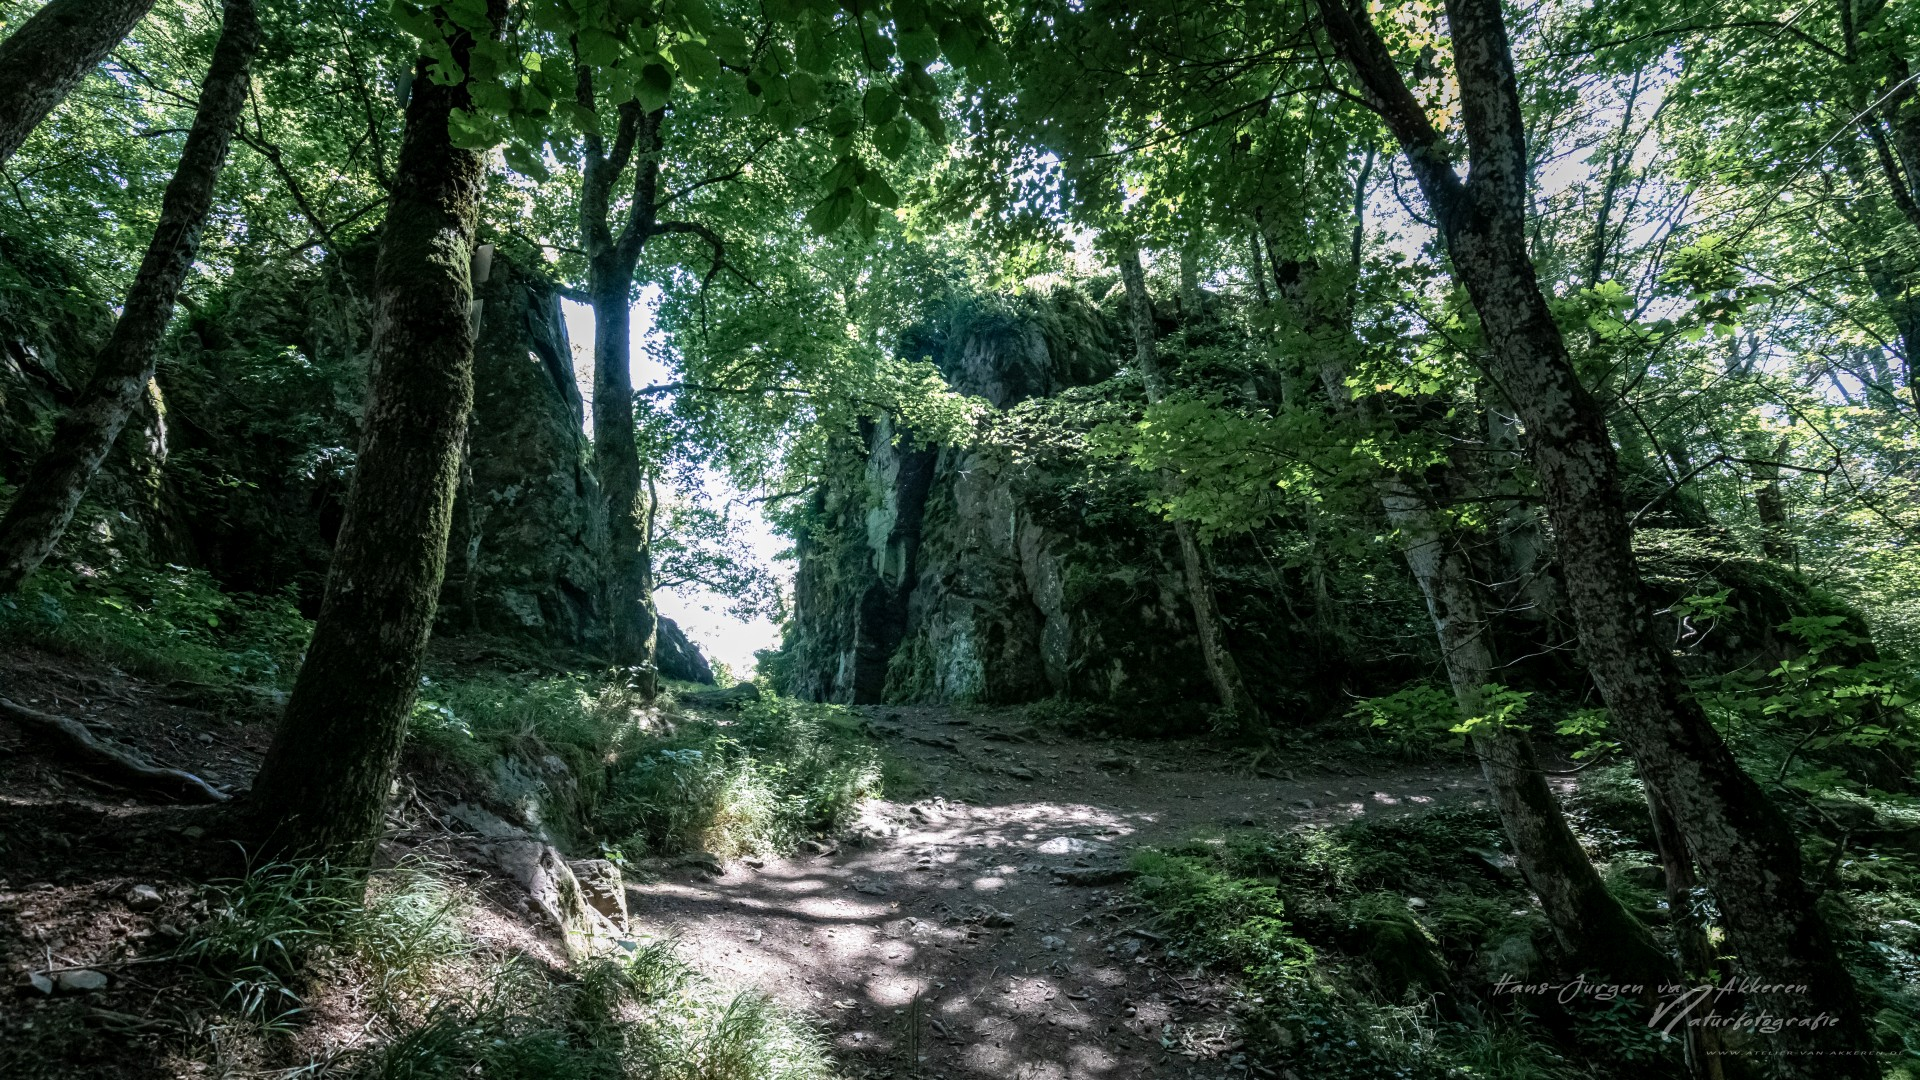
\includegraphics[width=\linewidth]{./figures/kybfelsen.png}
	\captionof{figure}{Die Burgruine Kybfelsen}
	\setlength{\parskip}{0.25cm}
	\vspace{0.15cm}

	Die \alert{Zähringer} waren ein bedeutendes schwäbisches Fürstengeschlecht des Mittelalters, das eine entscheidende Rolle bei der Gründung und Entwicklung von Freiburg im Breisgau spielte. Herzog Konrad von Zähringen gründete die Stadt im Jahr 1120 als Marktstadt, indem er einen Markt einrichtete und Kaufleuten Grundstücke zuwies. Die Zähringer bauten 1091 eine Burg auf dem Schlossberg, was die Stadtentwicklung maßgeblich förderte. Sie verliehen Freiburg weitreichende Freiheiten und Privilegien, wodurch die Stadt zum Zentrum ihres Herrschaftsgebiets wurde. Diese Maßnahmen trugen dazu bei den Handel und die wirtschaftliche Entwicklung der Region voranzutreiben. Nach dem Aussterben der Zähringer im Jahr 1218 ging Freiburg an die Grafen von Urach über, die sich fortan Grafen von Freiburg nannten. Dennoch blieb das positive Andenken an die Zähringer als Stadtgründer und Förderer in Freiburg erhalten. Ihr Erbe prägte nachhaltig die Entwicklung der Stadt und der gesamten Region zwischen Schwarzwald und Genfer See.

	% 1080 wurde in einem Bericht Otto von Freisings erstmals eine Burg Zähringen erwähnt, ein erster urkundlicher Nachweis befindet sich im Rotulus Sanpetrinus von 1128. Die Entstehungsgeschichte der Burg liegt im Dunkeln. Das darunterliegende Dorf Zähringen wurde 1008 erstmals in einer Schenkungsurkunde, der sogenannten Wildbannurkunde von König Heinrich II. an das Bistum Basel erwähnt, zusammen mit den Namen der Freiburger Stadtteile Herdern und Wiehre, der Nachbargemeinde Gundelfingen und anderer Orte im Breisgau.
\end{minipage}
\hspace{0.4cm}
\begin{minipage}[t]{0.32\textwidth}
	\vspace{0cm}
	\setlength{\parskip}{0.25cm}

	Ein kulinarischer Höhepunkt erwartet einen im \alert{Waldrestaurant St. Valentin}, wo regionale Spezialitäten und kühle Getränke zur Stärkung erworben werden können. \alert{St. Valentin} war ein christlicher Märtyrer aus dem 3. Jahrhundert, von dem es mehrere Überlieferungen gibt, darunter als ein Priester in Rom und ein Bischof in Terni. Er wird oft mit heimlichen Eheschließungen in Verbindung gebracht, was zu seiner späteren Hinrichtung führte. Die Assoziation mit dem Valentinstag und der Liebe entstand jedoch erst im Mittelalter und basiert mehr auf romantischen Traditionen als auf historischen Tatsachen.

	\includegraphics[width=\linewidth]{./figures/stvalentin.png}
	\captionof{figure}{Waldrestaurant St. Valentin aus der Vogelperspektive}
	\setlength{\parskip}{0.25cm}
	\vspace{0.15cm}

	% \footnote{
	% \tiny
	Der Freiburger Stadtteil \alert{St. Georgen} hat seinen Namen einem anderen christlichen Heiligen, dem heiligen Georg zu verdanken. Der Name leitet sich höchstwahrscheinlich von einer frühen Kapelle oder Kirche ab, die dem heiligen Georg geweiht war, da dieser Heilige im Mittelalter als wichtiger Schutzpatron galt. Es war damals üblich, Siedlungen nach Heiligen zu benennen, die als Schutzpatrone für die Region fungierten und die Sicherheit und den Segen Gottes für die Gemeinschaft repräsentierten.

	Der \alert{heilige Georg} war ein römischer Soldat und Märtyrer des 3. Jahrhunderts, der für seinen christlichen Glauben starb. Georg wurde aufgrund seines christlichen Glaubens verfolgt und schließlich während der Diokletianischen Christenverfolgung (ca. 303 n. Chr.) in Lydda (im heutigen Israel) als Märtyrer getötet. Da er sich weigerte, den christlichen Glauben aufzugeben und dem römischen Götterkult zu opfern, wurde er gefoltert und schließlich geköpft. Die Legende besagt, er habe einen Drachen besiegt und dadurch eine Stadt gerettet, wobei die Drachenlegende seine Rolle als Verteidiger des Guten und des christlichen Glaubens symbolisiert. Als Schutzpatron vieler Länder und Berufe, besonders der Ritter und Soldaten, steht er für Mut, Standhaftigkeit und den Einsatz für den Glauben.
	% }
\end{minipage}
\end{document}
